%  article.tex (Version 3.3, released 19 January 2008)
%  Article to demonstrate format for SPIE Proceedings
%  Special instructions are included in this file after the
%  symbol %>>>>
%  Numerous commands are commented out, but included to show how
%  to effect various options, e.g., to print page numbers, etc.
%  This LaTeX source file is composed for LaTeX2e.

%  The following commands have been added in the SPIE class 
%  file (spie.cls) and will not be understood in other classes:
%  \supit{}, \authorinfo{}, \skiplinehalf, \keywords{}
%  The bibliography style file is called spiebib.bst, 
%  which replaces the standard style unstr.bst.  

\documentclass[]{spie}  %>>> use for US letter paper
%%\documentclass[a4paper]{spie}  %>>> use this instead for A4 paper
%%\documentclass[nocompress]{spie}  %>>> to avoid compression of citations
%% \addtolength{\voffset}{9mm}   %>>> moves text field down
%% \renewcommand{\baselinestretch}{1.65}   %>>> 1.65 for double spacing, 1.25 for 1.5 spacing 
%  The following command loads a graphics package to include images 
%  in the document. It may be necessary to specify a DVI driver option,
%  e.g., [dvips], but that may be inappropriate for some LaTeX 
%  installations. 
\usepackage[]{graphicx}
\usepackage{url}
\usepackage[table, xcdraw]{xcolor}
\usepackage{subcaption}
\usepackage{amsmath}

\title{3D scanning by means of dual-projector structured light illumination} 

%>>>> The author is responsible for formatting the 
%  author list and their institutions.  Use  \skiplinehalf 
%  to separate author list from addresses and between each address.
%  The correspondence between each author and his/her address
%  can be indicated with a superscript in italics, 
%  which is easily obtained with \supit{}.

\author{Ying Yu\supit{a} and Daniel L. Lau\supit{a}
\skiplinehalf
\supit{a}University of Kentucky, 101 Main Building, Lexington, KY US; \\
%\supit{b}University of Kentucky, Address, Lexington, US
}

%>>>> Further information about the authors, other than their 
%  institution and addresses, should be included as a footnote, 
%  which is facilitated by the \authorinfo{} command.

\authorinfo{Further author information: (Send correspondence to Daniel L. Lau)\\Daniel L. Lau: E-mail: dllau@uky.edu, Telephone: 1 859 312 8047\\  Ying Yu: E-mail: yyu226@g.uky.edu} %, Telephone: +33 (0)1 98 76 54 32}
%%>>>> when using amstex, you need to use @@ instead of @
 

%%%%%%%%%%%%%%%%%%%%%%%%%%%%%%%%%%%%%%%%%%%%%%%%%%%%%%%%%%%%% 
%>>>> uncomment following for page numbers
% \pagestyle{plain}    
%>>>> uncomment following to start page numbering at 301 
%\setcounter{page}{301} 
 
  \begin{document} 
  \maketitle 

%%%%%%%%%%%%%%%%%%%%%%%%%%%%%%%%%%%%%%%%%%%%%%%%%%%%%%%%%%%%% 
\begin{abstract}
This paper introduces a dual-projector phase measuring profilometry that adds a second projector in a traditional structured light illumination system to improve the overall quality of the 3D scanning. With this method, two projectors are synchronized to a single camera, but each one projects structured light patterns of its unique frequency. The system performance benifits from a wider projection angle and a doubled light intensity. In particular, a detailed system implementation in hardware level is described. Moreover, the major difference between the phase unwrapping of dual-projector system and the single-projector system is discussed, and a LUT-based phase unwrapping scheme for this dual-projector phase measuring profilometry system is proposed. 
\end{abstract}

%>>>> Include a list of keywords after the abstract 

\keywords{Structured light illumination, phase measuring profilometry, dual-projector, phase unwrapping}

%%%%%%%%%%%%%%%%%%%%%%%%%%%%%%%%%%%%%%%%%%%%%%%%%%%%%%%%%%%%%
\section{Introduction}
\label{sec:intro}  % \label{} allows reference to this section
As one of the non-contact 3D shape measurement techniques, the structured light illumination (SLI) has been known for its high resolution and high speed~\cite{chen00}. Conventional SLI systems consist of one projector, one camera and one processing unit which is usually a computer. The projector presents patterns that are encoded with some information related to the pixel locations on the object to be measured. If the projection is on a flat surface, the patterns seen should be identical to its original design. However, with the presence of the non-planar object under the projection, what is actually seen from the camera is the distorted patterns on the surface of the object. By comparing and analyzing the distortion in the images taken by the camera, the 3D surface of the object can eventually be reconstructed in a processing unit.

Within the scope of this fundamental idea and system structure, a lot of research has been done over the past several decades~\cite{geng11}. Different practical implementations have been proposed, from pattern design to system calibration, then to the algorithms that are used to decode the captured patterns. One widely studied area is the one-shot SLI strategy in which only one static pattern is projected onto the object. It employs color pattern~\cite{wust91}, binary grid pattern~\cite{grin92}, gray-scale pattern~\cite{durd98} or even composite pattern~\cite{guan08}. Since there is only one image need to be processed for a scan, the 3D reconstruction can be completed fast. The one-shot strategy is ideal for high speed applications such as real time scanning. But in terms of accuracy, it is not so promising compared to some multi-shot SLI strategy in which the 3D reconstruction is derived by projecting a sequence of patterns and processing multiple images~\cite{blai03}.

According to the method of encoding the information containing the pixel location into the pattern, phase measuring profilometry (PMP)~\cite{srin85} is a subset of SLI techniques that acquires the depth value by translating the phase data from the projected patterns pixelwise. The PMP has some advantageous features including its insensitivity to ambient light and its high accuracy~\cite{guan03, hali89}. Higher frequency patterns have been introduced to PMP systems to reduce the effects of the noise and achieve higher accuracy~\cite{lijl03}. Nonetheless, higher frequency patterns also produces the phase ambiguity which requires the system to execute some extra computation called phase unwrapping~\cite{song18}. Furthermore, adding high frequency patterns increases the projection time as well as the number of images to be processed, which accordingly decreases the overall speed of the system. Liu \textit{et al}. proposed an ingenious dual-frequency pattern strategy which combines a high-frequency pattern and a unit-frequency pattern into one composite pattern~\cite{liuk10}, it improved the accuracy without increasing the scanning time.
\\
In this paper, we propose a dual-projector, dual-frequency SLI scheme and its practical implementation. Unlike the scanner presented by Jiang \textit{et al}.~\cite{jian18}, the proposed scanner projects patterns from both projectors simultaneously, which keeps the scan time the same versus a single projector scanner.  We also allow the projectors to be placed in any arbitrary arrangement with 3D point clouds generated from a single fused phase image instead of fusing to independently generated point clouds. Depending on the arrangements of projectors as illustrated in Fig.~\ref{Fig:10}, a dual-projector SLI scanner can be used to minimize occlusions~\cite{linj13} since a scan surface needs to be visible to at least one projector and the camera.  So placing projectors in opposition means a face, for example, can be illuminated from both sides.  Having two unique paths of light from projector to camera also creates new opportunities and challenges for overcoming the issue of multi-path~\cite{otoo16}. 

Placing projectors side-by-side can be used to achieve twice the luminance of a single projector. For instance, suppose the projectors we use are two identical Optoma ML750ST which has around 500 lumens each~\cite{lume70}, by using two projectors, we obtain a total 1000 lumens. Higher light intensity gives rise to the higher signal-to-noise ratios (SNR)~\cite{wangy10}, which makes the system less susceptible to sensor noise, consequently the system becomes more robust and accurate.

%%%%%%%%%%%%%%%%%%%%%%%%%%%%%%%%%%%%%%%%%%%%%%%%%%%%%%%%%%%%%%%%%%%%%%%%%%%%%%%%%%%%%%%%%%%%%%%%%%%%%%%%%%%%%%%%%%%%%%%%%%
\begin{figure}
\centerline{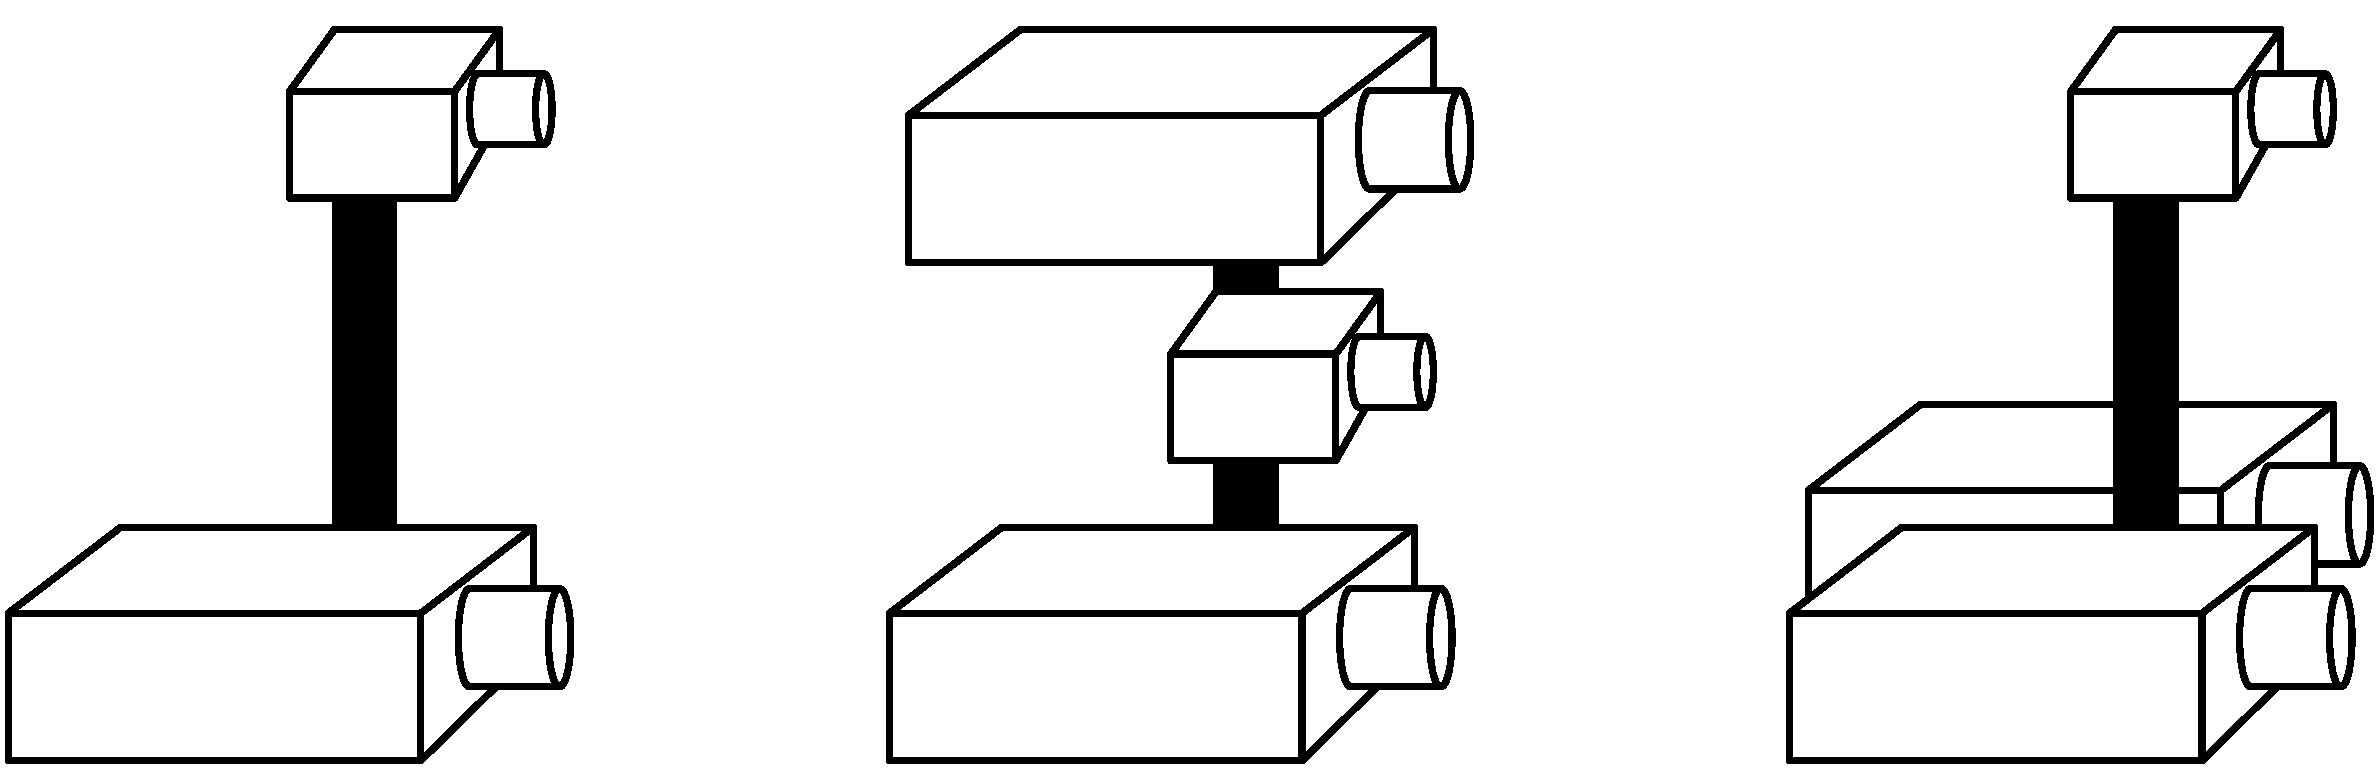
\includegraphics[width=5.0in]{Figures/Layouts}}
\vspace{0.1in}
\caption{Structured light scanners composed of (left) a single projector, (center) opposed dual-projectors for wrap around scanning, and (right) complementary dual-projectors for increased luminance.}
\label{Fig:10}
\end{figure} 
%%%%%%%%%%%%%%%%%%%%%%%%%%%%%%%%%%%%%%%%%%%%%%%%%%%%%%%%%%%%%%%%%%%%%%%%%%%%%%%%%%%%%%%%%%%%%%%%%%%%%%%%%%%%%%%%%%%%%%%%%%

Now in order for dual-projector SLI scanners to become practical, there are two fundamental problems that need to be addressed.  The first is the practical implementation of control logic to perfectly synchronize the projectors to a camera.  For this, we describe an FPGA-based controller using a commodity FPGA board to simultaneously drive two HDMI ports.  The advantage of this system is that it allows us to avoid the practical issues associated with modern GPUs as well as staying low cost.  The second problem that needs to be addressed is how to perform phase unwrapping when the phase images derive from separate projectors arbitrarily arranged.  Using the dual-frequency pattern scheme, we demonstrate using a unit-frequency phase image from one projector to unwrap the high-frequency phase image in the second, opposed projector, using a look-up table-based operation ideally suited for GPUs. This real-time approach is highly flexible and can be used to replace phase unwrapping schemes such as the Chinese remainder technique of Xia \textit{et al}. ~\cite{xiax07}.

\section{Dual-frequency Phase Measuring Profilometry}
The dual-frequency pattern scheme was initially proposed by Liu \textit{et al}.\cite{liuk10}, it is essentially  an improved derivation of the phase measuring profilometry~\cite{hali89}. In the the traditional PMP a series of phase-shifting sinusoidal fringe patterns are projected onto the object to be measured, the fringe patterns can be either horizontal or vertical, the presence of the object distorts the patterns, then by analyzing the phase values in the deformed pattern images, the 3D depth values can be obtained.

Suppose the phase-shifting patterns are vertical, which indicates that all the pixels in a same row have the identical intensity, and from top to bottom the value of intensities in each row form a sinusoidal function. Therefore, this kind of PMP patterns can be generalized as:
 \begin{equation} \label{eq:1.1}
  	I^p_n(x^p, y^p) = A^p + B^p\cos\left(2\pi f y^p - \frac{2\pi n}{N}\right),
  \end{equation}
where $I^p_n$ is the intensity of the pixel at the coordinate $(x^p, y^p)$ from the projector's point of view; $A^p$ is background intensity which is considered as a constant; $B^p$ is another constant which represents the fringe contrast compared to the background; $f$ is the frequency of the fringe pattern set which is equal to the number of sinusoidal periods from top to the bottom of the projected patterns; $N$ is the total number of the phase-shifting patterns of the same frequency in a set, $n$ is the current number of the pattern within the range of $[0, N-1]$.

On the camera's side, the image of  the object under the projection of each unique PMP pattern is captured as part of the data to reconstruct the 3D profile of the object. So the projected scene of the object can be described as Eq.~\eqref{eq:1.2} from the camera's point of view, 
 \begin{equation} \label{eq:1.2}
  	I^c_n(x^c, y^c) =  A^c(x^c, y^c) + B^c(x^c, y^c)\cos\left(\phi(x^c, y^c) - \frac{2\pi n}{N}\right),
  \end{equation}
where $I^c_n$ is the intensity of the given pixel $(x^c, y^c)$ in the camera's coordinates system; $A^c(x^c, y^c)$ is the average intensity of the given pixel over the $N$ patterns; $B^c$ can be considered as the average intensity of the PMP pattern seen by the camera, so for any given pixel $(x^c, y^c)$ in a pattern set $[0, N-1]$, $A^c$ and $B^c$ are both constant, furthermore, $B^c(x^c, y^c)$ can be derived from Eq.~\eqref{eq:1.2} as:
  \begin{equation} \label{eq:1.3}
  	B^c(x^c, y^c) = \frac{2}{N}\sqrt{\left[\sum_{n=0}^{N-1}I_n^c(x^c, y^c)\sin (\frac{2\pi n}{N})\right]^2 + \left[\sum_{n=0}^{N-1}I_n^c(x^c, y^c)\cos (\frac{2\pi n}{N})\right]^2}.
  \end{equation}
In Eq.~\ref{eq:1.2}, there is another important constant $\phi$ for any given pixel $(x^c, y^c)$ in a given pattern set $[0, N-1]$, it is the phase value $\phi (x^c, y^c)$ of the distorted fringe patterns that is eventually used to calculate the corresponding depth value of the object. The expression of $\phi (x^c, y^c)$ can be inferred from Eq.~\eqref{eq:1.3} as:
  \begin{equation} \label{eq:1.4}
  	\phi (x^c, y^c) = \frac{1}{2\pi}\left(\arctan \frac{\sum_{n=0}^{N-1} I^c_n(x^c, y^c)\sin(\frac{2\pi n}{N})}{\sum_{n=0}^{N-1} I^c_n(x^c, y^c)\cos(\frac{2\pi n}{N})} + \pi\right),
  \end{equation}
in Eq.~\eqref{eq:1.4}, the phase value $\phi (x^c, y^c)$ is converted to a range of $[0, 1]$.\\
The dual-frequency pattern scheme adds a second sinusoidal component to the phase-shifting patterns, as a result, the total number of patterns is still $N$, but each pattern has two sinusoidal components, one is of unit frequency $f_u$, the other is of a high frequency $f_h$ that is used to reduce the impact of noises in the system. If we extend the single-frequency PMP pattern above to the dual-frequency, the intensities of the row pixels from top to bottom would be like an amplitude modulation in which the $f_u$ is frequency of the modulating signal and $f_h$ is the frequency of the carrier wave. According to Liu \textit{et al}., from the projector's point of view, the new dual-frequency pattern is expressed as:
  \begin{equation} \label{eq:1.5}
  	I^p_n(x^p, y^p) = A^p + B^p_1\cos\left(2\pi f_h y^p - \frac{2\pi n}{N}\right) + B^p_2\cos\left(2\pi f_u y^p - \frac{4\pi n}{N}\right),
  \end{equation}
where the $I^p_n$ is the intensity of the pixel $(x^p, y^p)$ in the $n^{th}$ pattern. Similarly the intensity equation of the camera coordinates used for reconstruction becomes:
 \begin{equation} \label{eq:1.6}
  	I^c_n(x^c, y^c) =  A^c(x^c, y^c) + B^c_1(x^c, y^c)\cos\left(\phi_h(x^c, y^c) - \frac{2\pi n}{N}\right) + B^c_2(x^c, y^c)\cos\left(\phi_u(x^c, y^c) - \frac{4\pi n}{N}\right).
  \end{equation}
Likewise the $B^c_1$, $B^c_2$ and $\phi_h$, $\phi_u$ can be derived from Eq.~\eqref{eq:1.3} and Eq. \eqref{eq:1.4} respectively,
  \begin{equation} \label{eq:1.7}
  	B^c_m(x^c, y^c) = \frac{2}{N}\sqrt{\left[\sum_{n=0}^{N-1}I_n^c(x^c, y^c)\sin (m\frac{2\pi n}{N})\right]^2 + \left[\sum_{n=0}^{N-1}I_n^c(x^c, y^c)\cos (m\frac{2\pi n}{N})\right]^2},
  \end{equation}
where $m = 1\: or\: 2$ in this case,
 \begin{equation} \label{eq:1.8}
  	\phi_h (x^c, y^c) = \frac{1}{2\pi}\left(\arctan \frac{\sum_{n=0}^{N-1} I^c_n(x^c, y^c)\sin(\frac{2\pi n}{N})}{\sum_{n=0}^{N-1} I^c_n(x^c, y^c)\cos(\frac{2\pi n}{N})} + \pi\right),
  \end{equation}
 \begin{equation} \label{eq:1.9}
  	\phi_u (x^c, y^c) = \frac{1}{2\pi}\left(\arctan \frac{\sum_{n=0}^{N-1} I^c_n(x^c, y^c)\sin(\frac{4\pi n}{N})}{\sum_{n=0}^{N-1} I^c_n(x^c, y^c)\cos(\frac{4\pi n}{N})} + \pi\right).
  \end{equation}
Now in Eq.~\eqref{eq:1.8} and \eqref{eq:1.9}, $\phi_h$ and $\phi_u$ are confined within $[0, 1]$; however, the actual range of $\phi_h$ is $[0, f_h]$, the  $\phi_h$ is called the wrapped phase. Unwrapping the $\phi_h$ to $\tilde{\phi}_h \in [0, f_h]$ can lead to a more accurate conversion from phase to depth.  In order to obtain $\tilde{\phi}_h$, the value of $\phi_u$ is used as the following equation shows,
  \begin{equation} \label{eq:1.10}
	 \tilde{\phi}_h = \phi_h + \lfloor f_h \phi_u - \phi_h + 0.5 \rfloor,
  \end{equation}
where the $\lfloor \rfloor$ is the symbol of floor function which outputs the greatest integer less than or equal to the value enclosed.

Now that we have unambiguous, unwrapped phase term, $\tilde{\phi}_h$, we can derive the 3D point from our scan according to Liu \textit{et al}. ~\cite{liuk10}:
\begin{equation}\label{eq:1.11}
	Z^w = M_z(x^c, y^c) + \frac{N_z(x^c, y^c)}{C(x^c, y^c) \tilde{\phi}_h + 1},
\end{equation}
and then
\begin{equation}\label{eq:1.12}
	X^w = E_x(x^c, y^c)Z^w + F_x(x^c, y^c),
\end{equation}
\begin{equation}\label{eq:1.13}
	Y^w = E_y(x^c, y^c)Z^w + F_y(x^c, y^c).
\end{equation}
where the coefficients $M_z$, $N_z$, $E_x$, $E_y$, $F_x$, $F_y$ and $C$ are determined during calibration of the projector and cameras lenses, assuming pin-hole lens models.


\section{Dual-Projector Phase Measuring Profilometry}
In this paper, we apply the dual-frequency PMP to a dual-projector system in which the SLI patterns in Eq.~\eqref{eq:1.5} are jointly generated by two separate projectors A and B. The projector A produces the high frequency component while the projector B only produces the unit frequency component. Thus their intensity equations can be expressed respectively as:
   \begin{equation} \label{eq:1.14}
  	I^{p_a}_n(x^{p_a}, y^{p_a}) = A^{p_a} + B^{p_a}_1\cos\left(2\pi f_h y^{p_a} - \frac{2\pi n}{N}\right), and 
  \end{equation}
   \begin{equation} \label{eq:1.15}
  	I^{p_b}_n(x^{p_b}, y^{p_b}) = A^{p_b} + B^{p_b}_2\cos\left(2\pi f_u y^{p_b} - \frac{4\pi n}{N}\right).
  \end{equation}
During the reconstruction process, the Eq.~\eqref{eq:1.6} to Eq.~\eqref{eq:1.9} remain the same as what they are in the single-projector system, because the dual-projector system does not make it much different from the camera's point of view. However, the Eq.~\eqref{eq:1.10} is not applicable for the dual-projector system anymore. 

%%%%%%%%%%%%%%%%%%%%%%%%%%%%%%%%
%replacement equation 10
%we populate this table based on data collected during calibration...
Instead, we use a lookup table (LUT) to acquire the unwrapped phase, as Eq.~\eqref{eq:1.16} shows,

\begin{equation} \label{eq:1.16}
  	\tilde{\phi}_d(x^c, y^c) = LUT[x^c, y^c, \phi_{p_b}] + \phi_{p_a},
  \end{equation}
where the $\tilde{\phi}_d$ is the unwrapped phase of the pixel $(x^c, y^c)$, $\phi_{p_a}$ is the phase derived from projector A and $\phi_{p_b}$ is the phase derived from projector B.
The LUT is populated from the data collected during calibration.
%%%%%%%%%%%%%%%%%%%%%%%%%%%%%%%%

%<<<<<<< HEAD
The procedure for calibrating our scanner is illustrated in Fig.~\ref{Fig:20} and involves sweeping a rigid, flat checkerboard pattern in correspondence with the $XY$-plane and moving in fixed, small-steps through the scan volume from the nearest plane where $Z = Z_{min}$ to the farthest plane at $Z = Z_{max}$.  The physical moving of the checkerboard pattern is performed using a motorized rail like the Velmex Bi-slide and VXM controller.  These rails can be configured to move with a positional accuracy of 0.076~mm and repeatability of 0.005~mm.  The specific checkerboard pattern that we use the CalTag calibration target introduced by Atcheson \textit{et al}.~\cite{atch10} where, inside each square, is a unique 16-bit codeword identifying and absolute world $(X_w,Y_w)$ coordinates of each squares four corners.
%=======
%%%%%%%%%%%%%%%%%%%%%%%%%%%%%%%%%%%%%%%%%%%%%%%%%%%%%%%%%%%%%%%%%%%%%%%%%%%%%%%%%%%%%%%%%%%%%%%%%%%%%%%%%%%%%%%%%%%%%%%%%%
%%%%%%%%%%%%%%%%%%%%%%%%%%%%%%%%%%%%%%%%%%%%%%%%%%%%%%%%%%%%%%%%%%%%%%%%%%%%%%%%%%%%%%%%%%%%%%%%%%%%%%%%%%%%%%%%%%%%%%%%%%
%%%%%%%%%%%%%%%%%%%%%%%%%%%%%%%%%%%%%%%%%%%%%%%%%%%%%%%%%%%%%%%%%%%%%%%%%%%%%%%%%%%%%%%%%%%%%%%%%%%%%%%%%%%%%%%%%%%%%%%%%%
\section{Calibration}
The procedure for calibrating our scanner is illustrated in Fig.~\ref{Fig:20} and involves sweeping a rigid, flat checkerboard pattern, in correspondence with the $XY$-plane, in fixed, small-steps through the scan volume from the nearest plane at $Z = Z_{min}$ to the farthest plane at $Z = Z_{max}$.  The physical moving of the checkerboard pattern is performed using a motorized rail like the Velmex Bi-slide and VXM controller.  These rails can be configured to move with a positional accuracy of 0.076~mm and repeatability of 0.005~mm.  The specific checkerboard pattern that we use is the CalTag calibration target introduced by Atcheson et al~\cite{atch10} where, inside each square, is a unique 16-bit codeword identifying and absolute world coordinates,  $(X_w,Y_w)$, of each square's four corners.
%>>>>>>> 716b5f75bdda6aa6bf4630801fbe0c1071de81a3

%%%%%%%%%%%%%%%%%%%%%%%%%%%%%%%%%%%%%%%%%%%%%%%%%%%%%%%%%%%%%%%%%%%%%%%%%%%%%%%%%%%%%%%%%%%%%%%%%%%%%%%%%%%%%%%%%%%%%%%%%%
\begin{figure}[!t]
\centerline{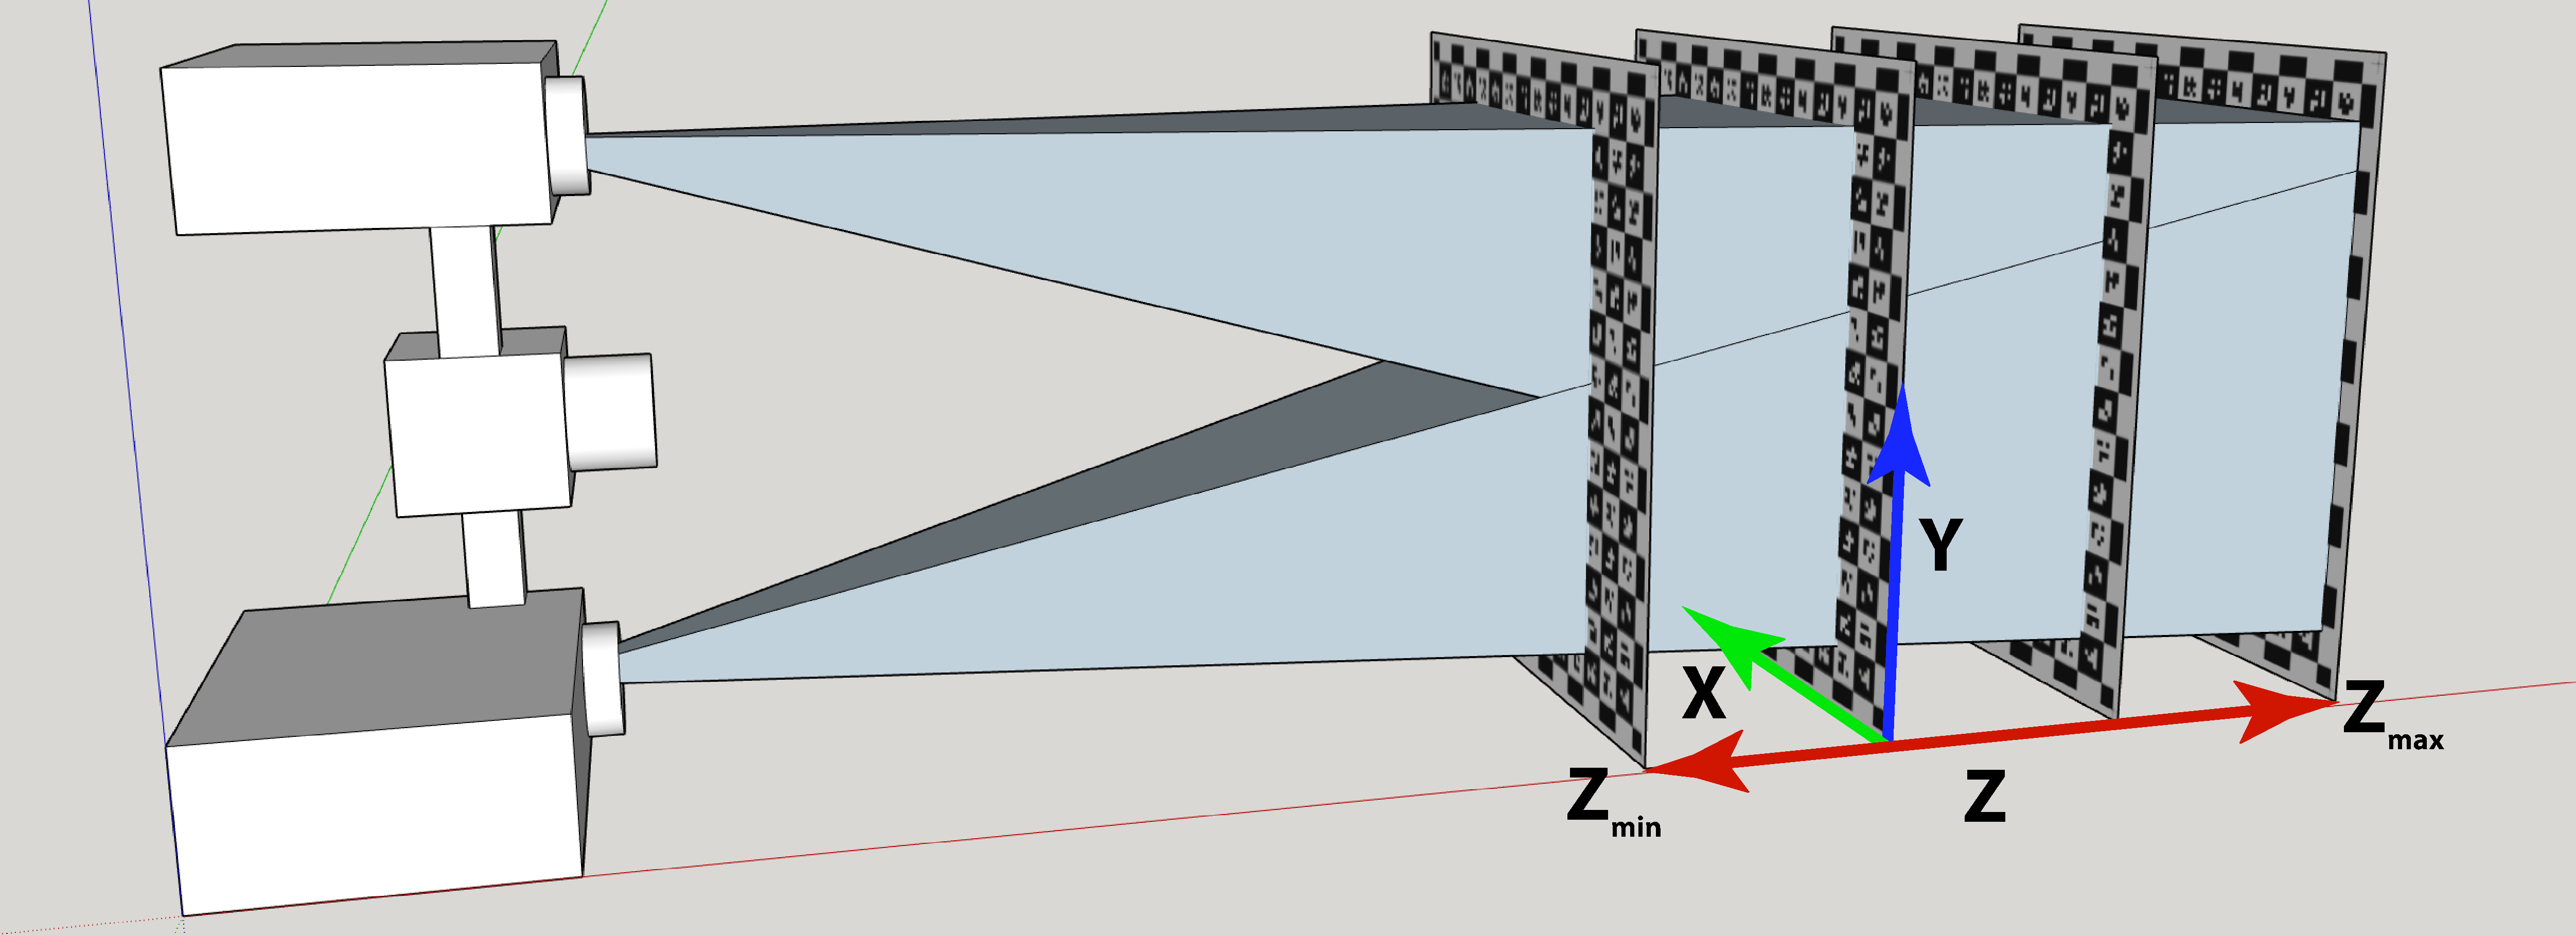
\includegraphics[width=6.6in]{Figures/SLICalibrationDual}}
\vspace{0.1in}
\caption{Illustration showing dual-projector scanner calibration.}
\label{Fig:20}
\end{figure} 
%%%%%%%%%%%%%%%%%%%%%%%%%%%%%%%%%%%%%%%%%%%%%%%%%%%%%%%%%%%%%%%%%%%%%%%%%%%%%%%%%%%%%%%%%%%%%%%%%%%%%%%%%%%%%%%%%%%%%%%%%%

As stated above, the calibration procedure involves iteratively moving the CalTag target along the Z-axis from $Z_{min}$ to $Z_{max}$ such that, at each step, we perform a structured light scan with each camera pixel defined according to:
\begin{equation}
%<<<<<<< HEAD
I_c[x^c, y^c, k] = [X_w[x^c, y^c, k], Y_w[x^c, y^c, k], Z_w[x^c, y^c, k], P_a[x^c, y^c, k], P_b[x^c, y^c, k]]
\label{calEqn}
\end{equation}
where $x^c$ and $y^c$ are the pixel’s column and row coordinates; $k$ is the step index for the current scan; $X_w[x^c, y^c, k]$ and $Y_w[x^c, y^c, k]$ are the CalTag grid coordinate at the intersection of the CalTag target’s surface and the camera pixel’s line-of-sight; $Z_w[x^c, y^c, k]$ is the Z-position of the rail; and $P[x^c, y^c, k]$ is the phase value of the projected PMP sequence in the line-of-sight of the camera pixel.  Once complete, we then have a 3D texture composed of a stack of 4-color digital images that are the height and width of our camera and $K$ layers deep with $P[x^c, y^c, k]$ ranging from $P_{min}[x^c, y^c]$ to $P_{max}[x^c, y^c]$ as $Z_w[x^c, y^c, k]$ ranges from $Z_{min}[x^c, y^c]$ to $Z_{max}[x^c, y^c]$.

%%%%%%%%%%%%%%%%%%%%%%%%%%%%%%%%%%%%%%%%%%%%%%%%%%%%%%%%%%%%%%%%%%%%%%%%%%%%%
%NOW LET"S LOOK AT A PLOT OF PA VS PB IN THE DUAL PROJECTOR SYSTEM AND COMPARE IT WITH A PLOT OF PLOW VS PHIGH IN THE SINGLE PROJECTOR SYSTEM
%IN LIGHT OF THIS PLOT, WE POPULATE THE LUT FROM EQN. (NEW 10) SUCH THAT LUT[PLOW] = FUNCTION EQUAL TO PHIGH
Fig.~\ref{Fig:3} illustrates the relationship between the $\phi_f$ and $\phi_h$ for the single-projector PMP system (left) and the dual-projector PMP system (right) respectively.
\begin{figure}[!t]
  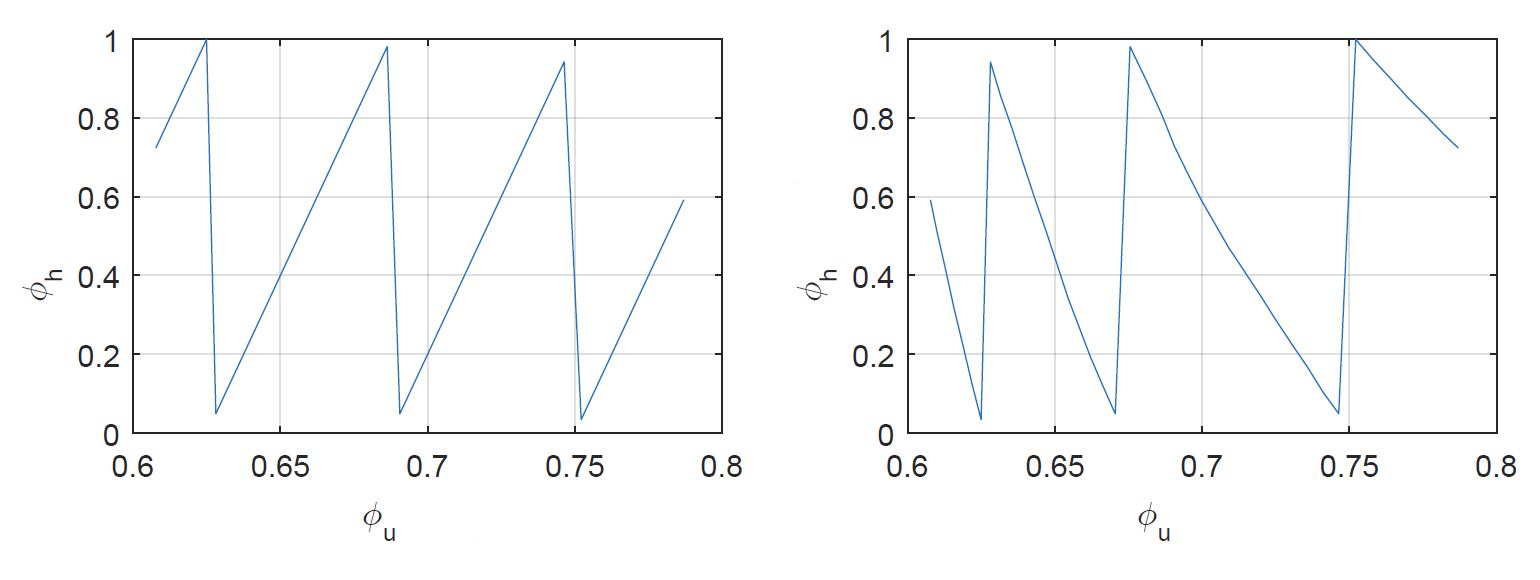
\includegraphics[width=\linewidth]{phase.png}
  \caption{$\phi_f$ vs. $\phi_u$ in single-projector system (left) and dual-projector system (right)}
  \label{Fig:3}
\end{figure}
%%%%%%%%%%%%%%%%%%%%%%%%%%%%%%%%%%%%%%%%%%%%%%%%%%%%%%%%%%%%%%%%%%%%%%%%%%%%%




















\section{System Implementation}
Our FPGA-based dual-projector Structured Light Illumination (SLI) system generates two synchronized SLI patterns which are then fed to two projectors via HDMI. Meanwhile, the projectors and the camera need to be synchronized to ensure that the camera images are taken at the right timing. A photo of our system and the system diagram are shown in Fig.~\ref{fig:sub1} and Fig.~\ref{fig:sub2}. The two SLI pattern generators output two synchronized phase-shifting fringe patterns which are later encoded into TMDS data streams by the HDMI transmitters and eventually move to projectors. 

%\begin{figure}
 %  \begin{center}
  % \begin{tabular}{c}
   %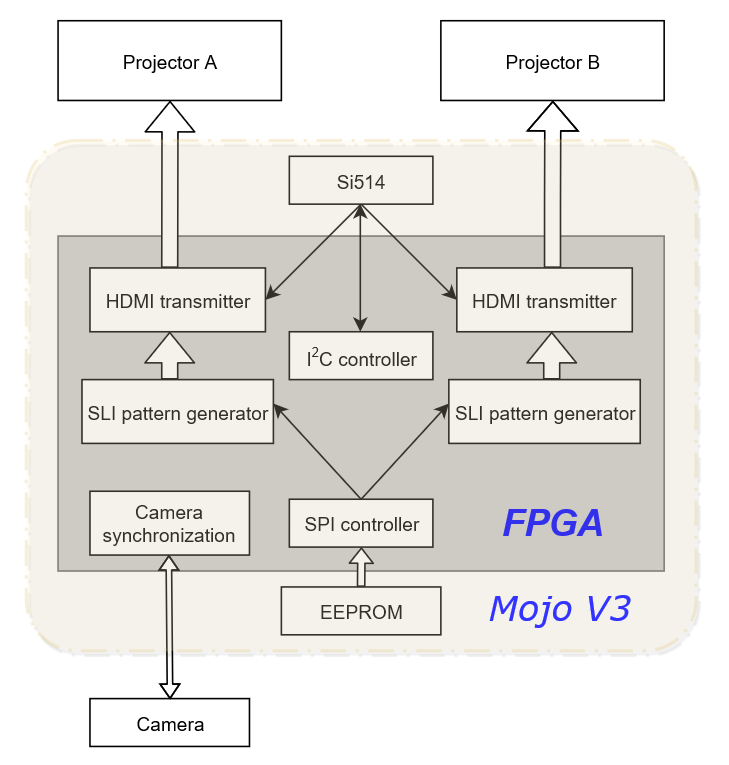
\includegraphics[height=7cm]{sysdgv2.png}
   %%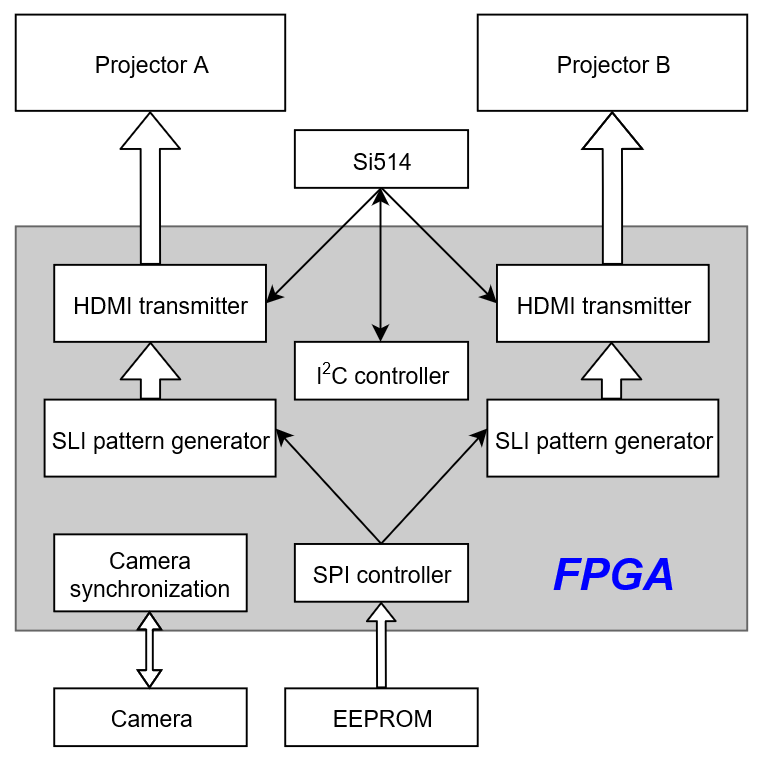
\includegraphics[width=\linewidth]{sysdg.png} 
   %\end{tabular}
   %\end{center}
   %\caption{System diagram}
   %\label{Fig:1}
   %\end{figure} 

\begin{figure}
\centering
\begin{subfigure}{.5\textwidth}
  \centering
  %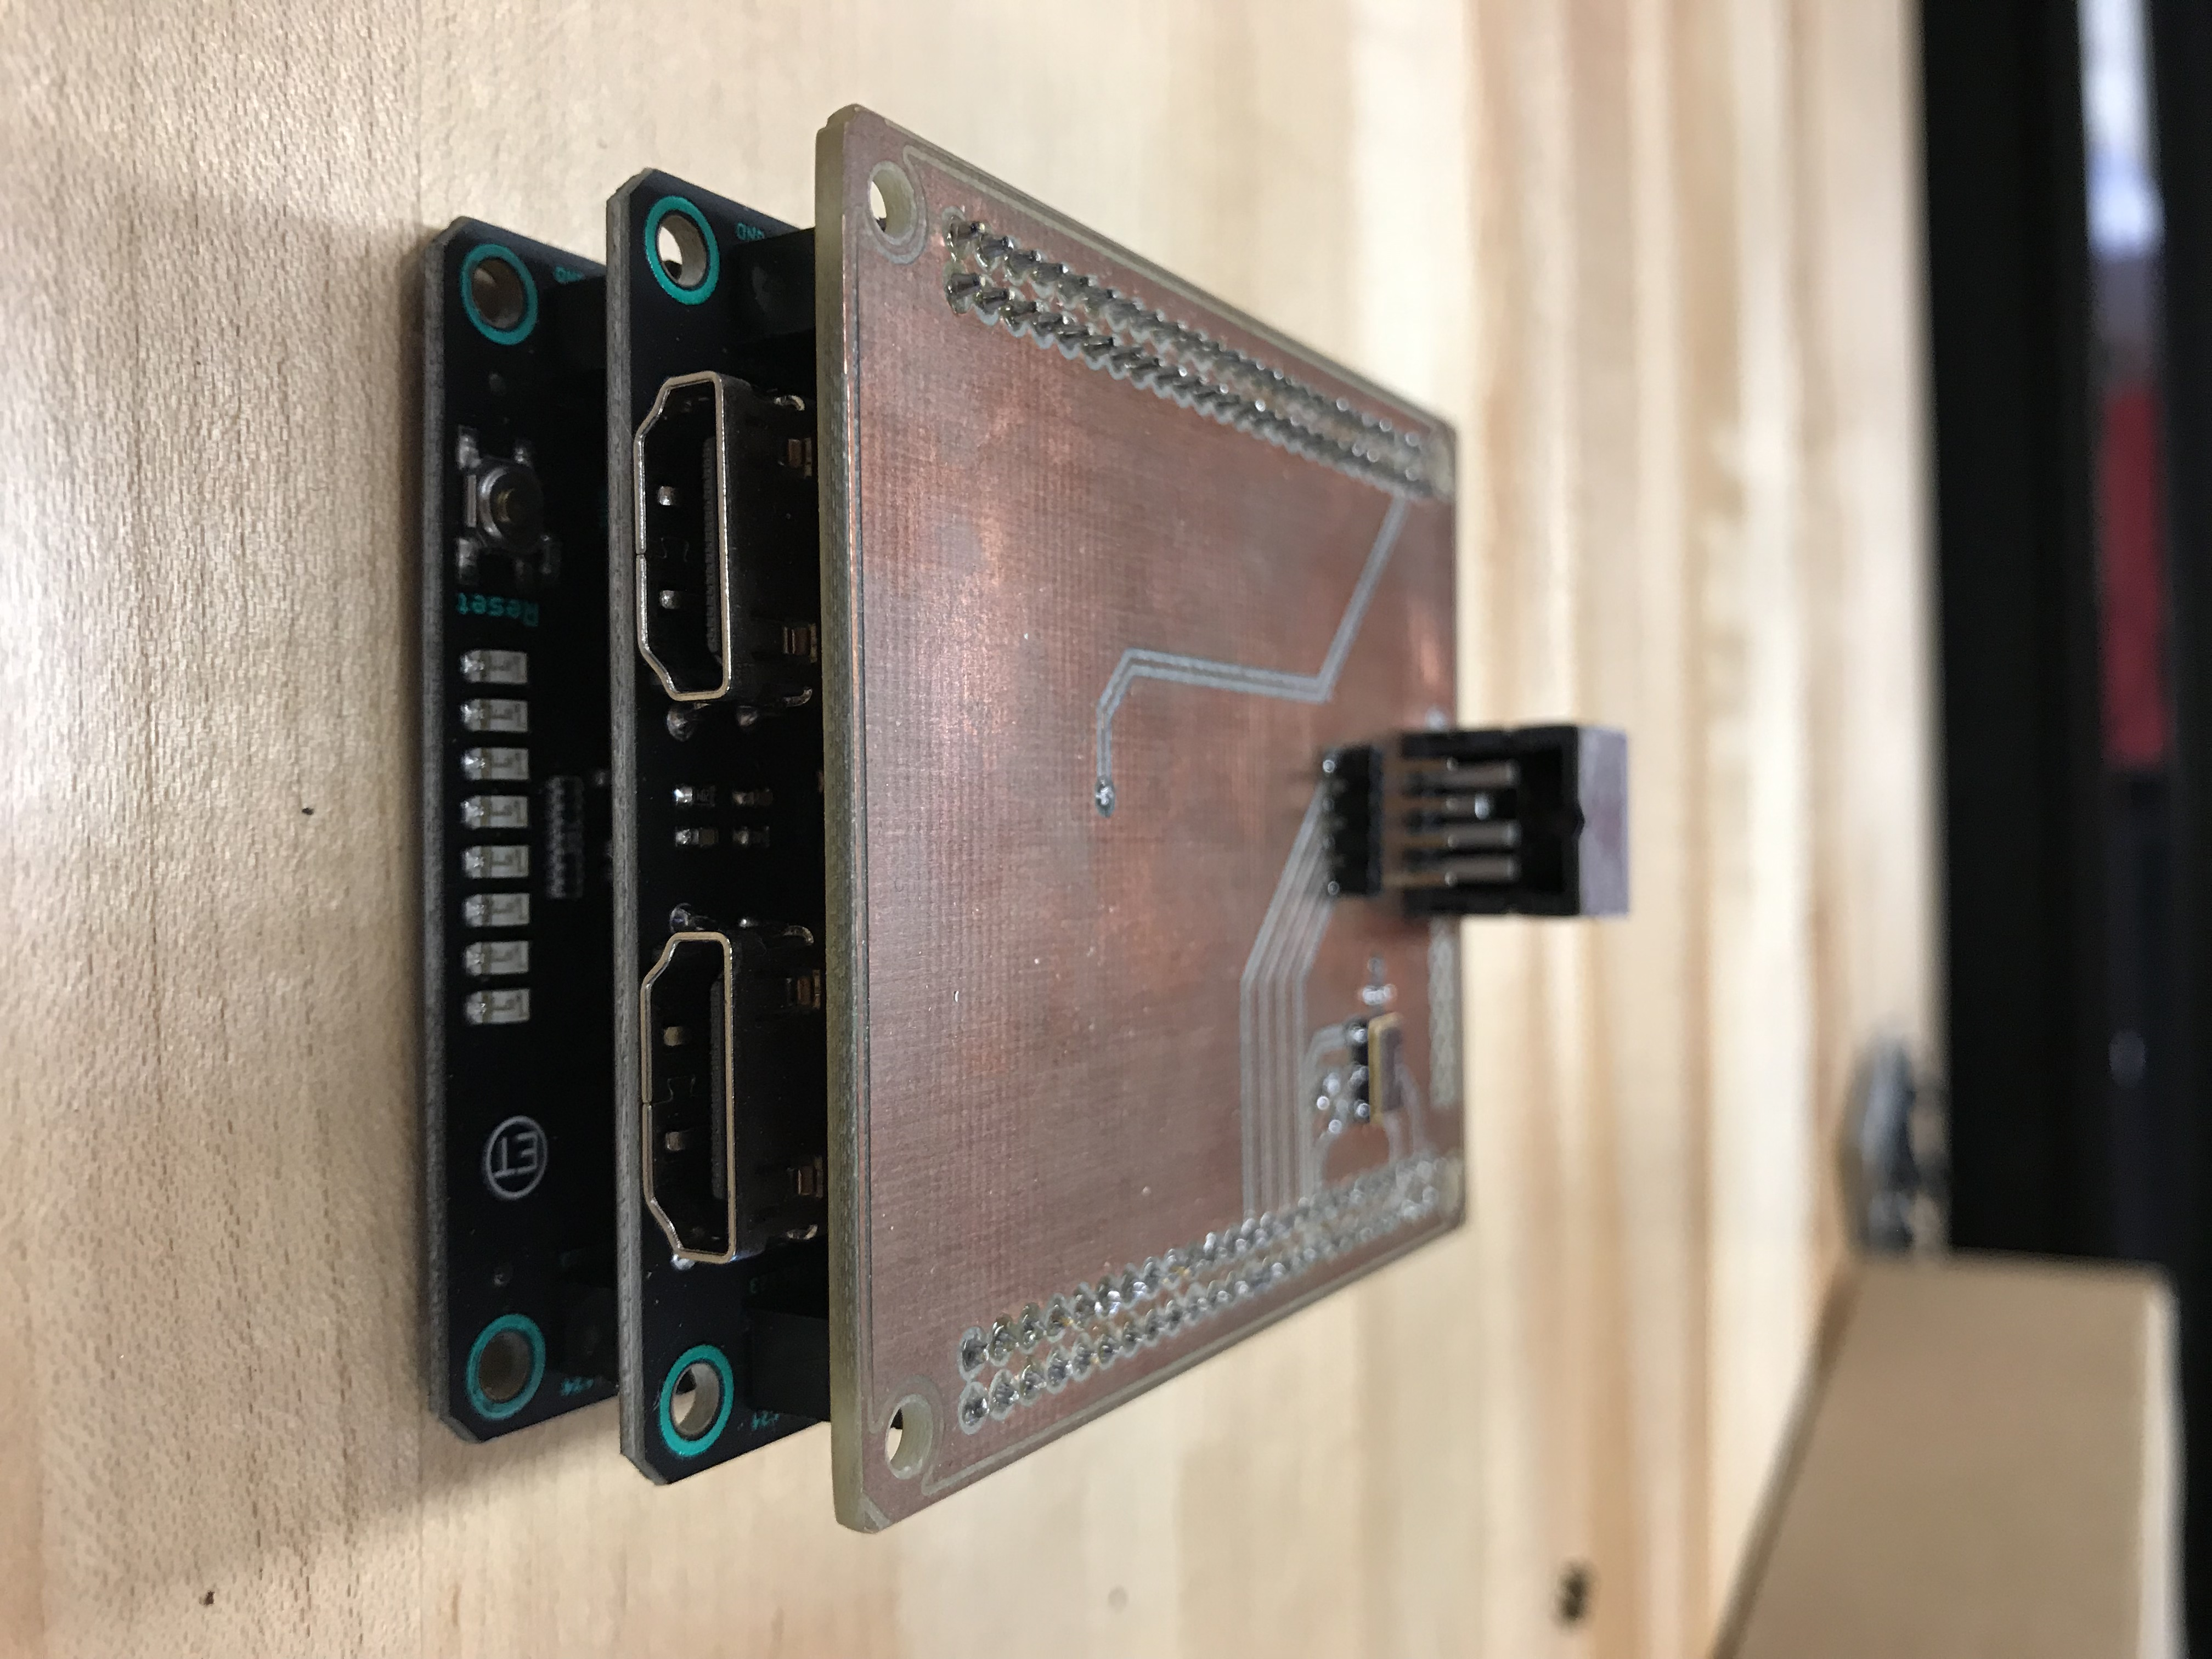
\includegraphics[width=.5\linewidth]{mojo.jpg}
  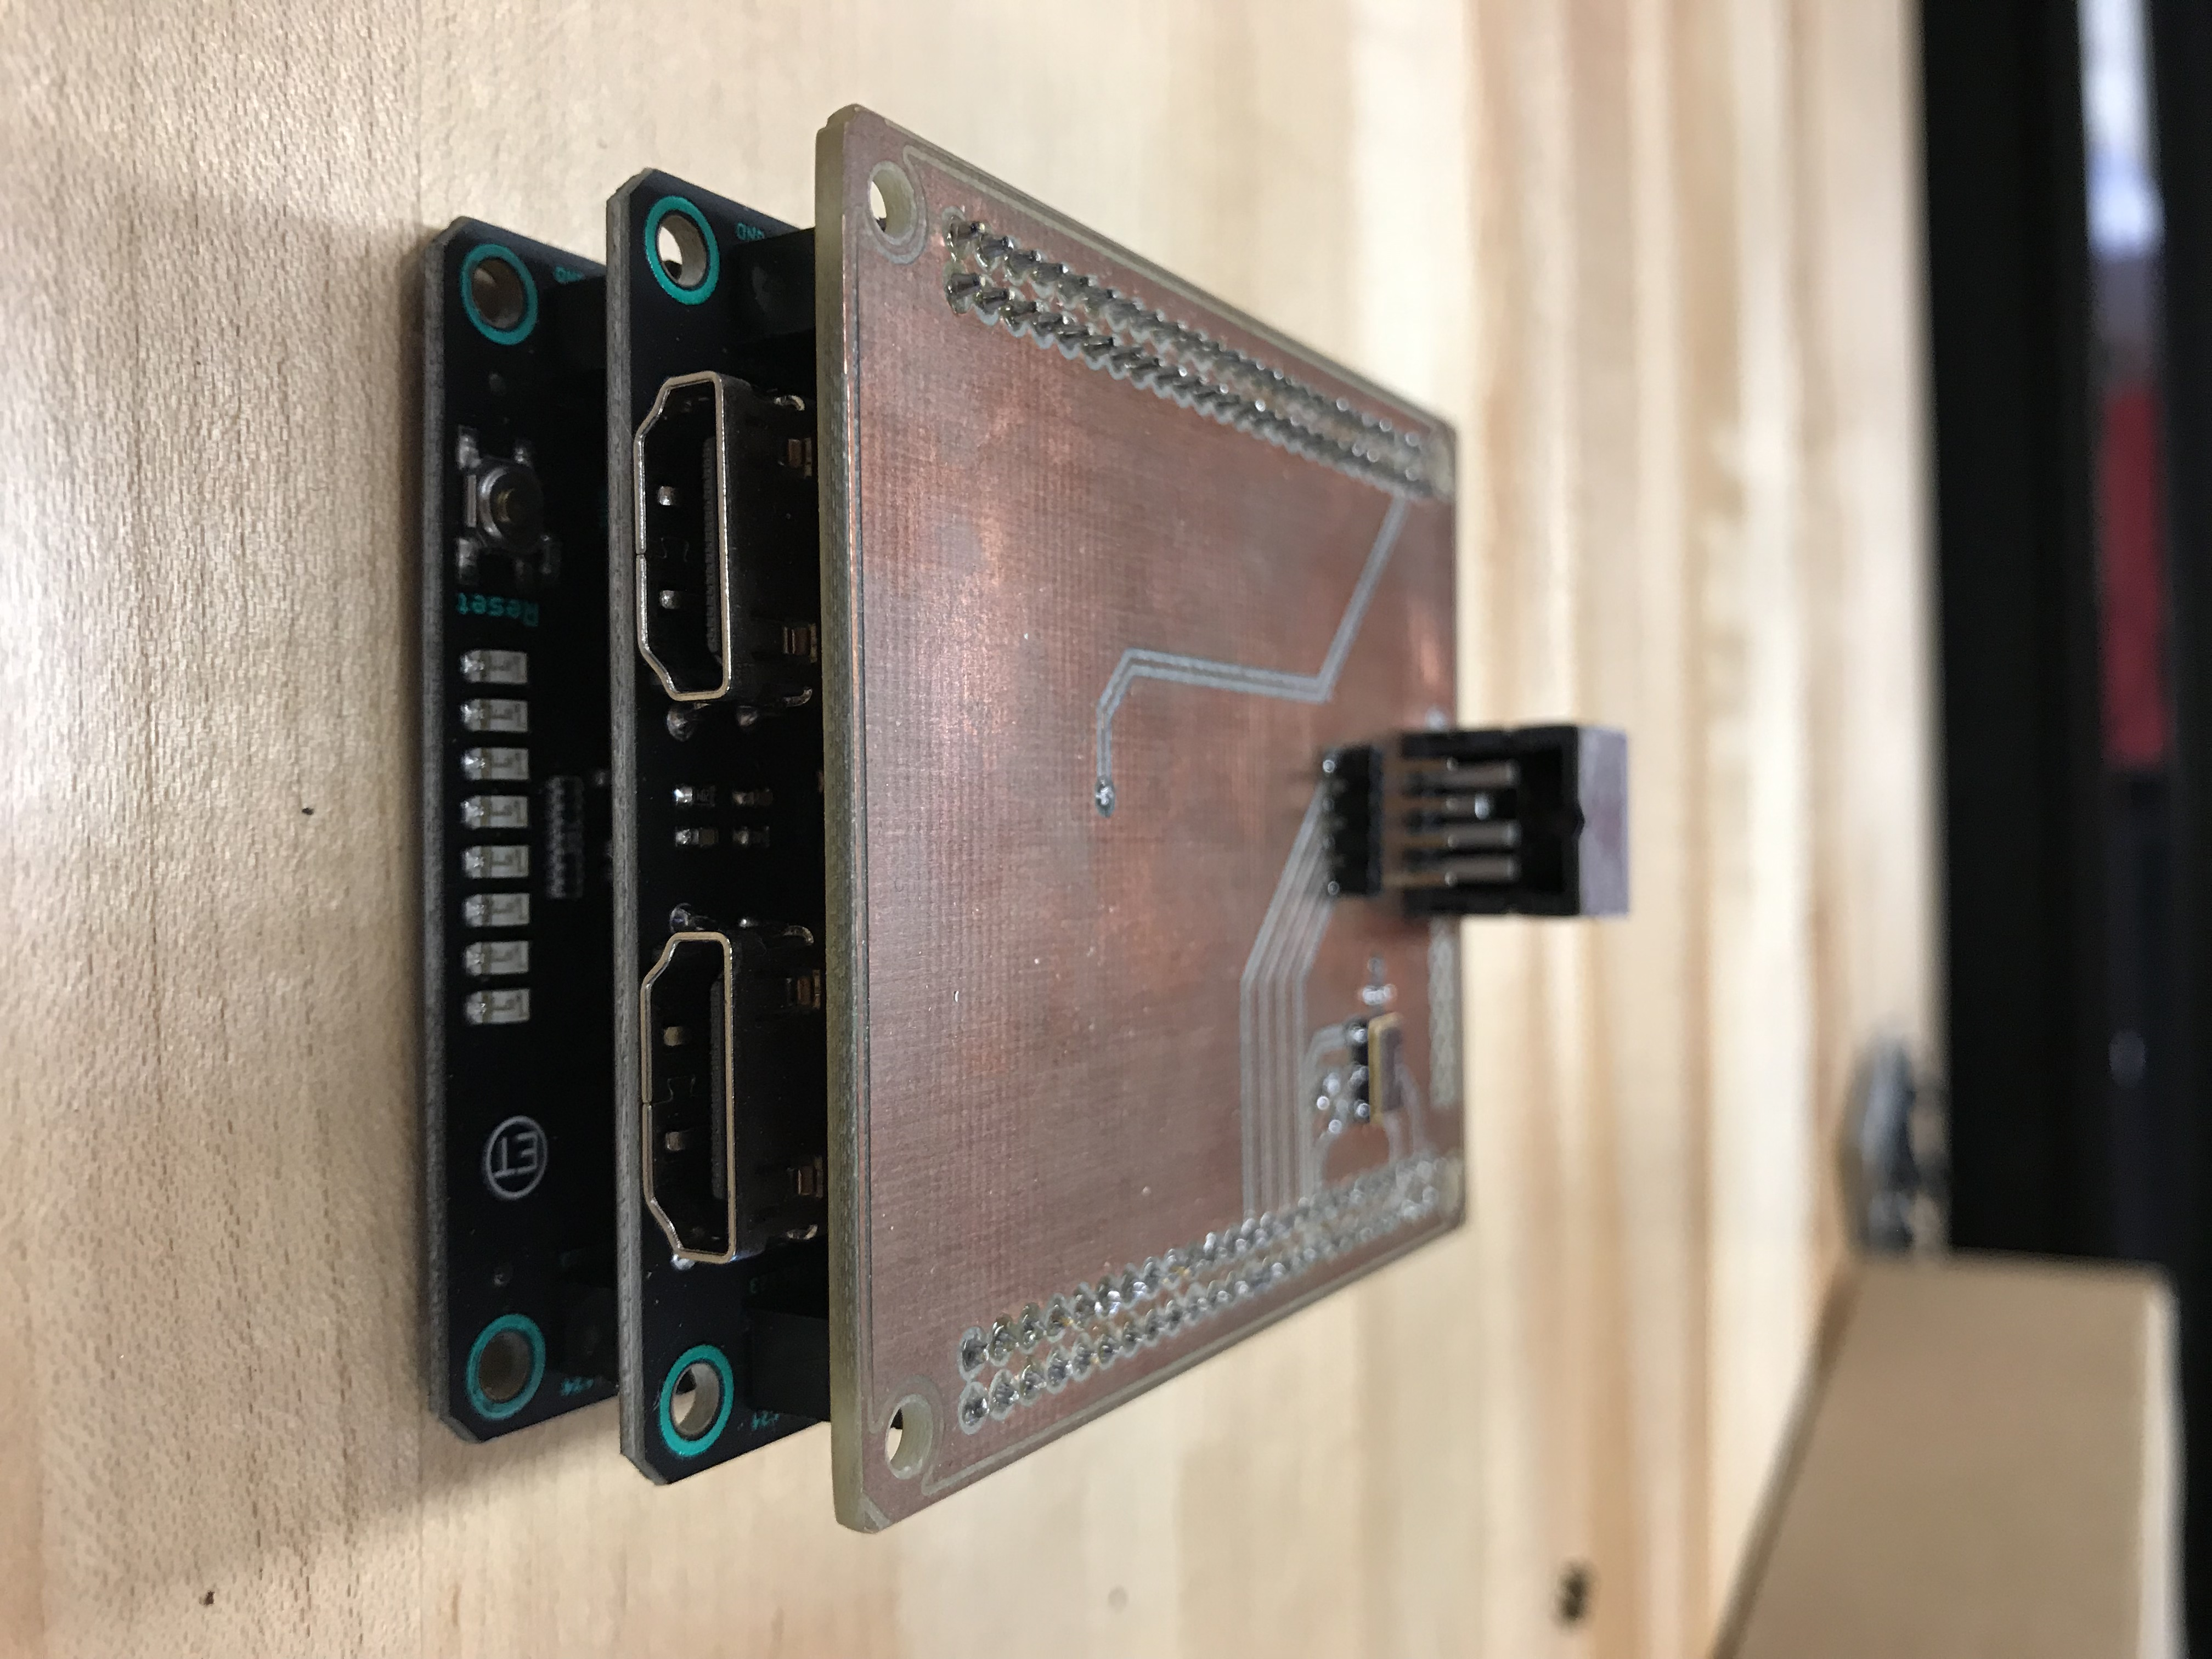
\includegraphics[height=6cm, angle=90]{mojo.jpg}
  \caption{A photo of the system}
  \label{fig:sub1}
\end{subfigure}%
\begin{subfigure}{.5\textwidth}
  \centering
  %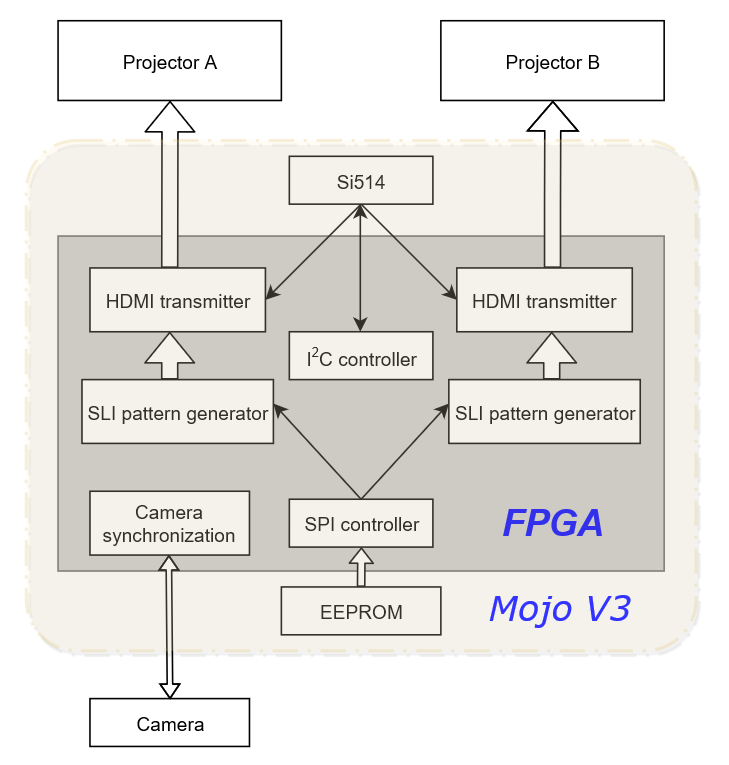
\includegraphics[width=.5\linewidth]{sysdgv2.png}
   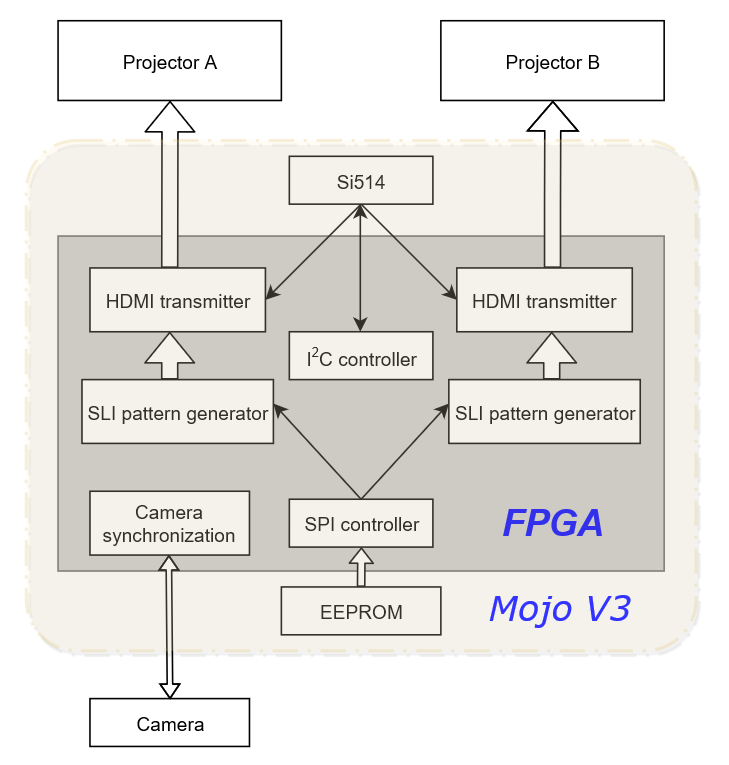
\includegraphics[height=8cm]{sysdgv2.png}
  \caption{System diagram}
  \label{fig:sub2}
\end{subfigure}
\caption{Our dual-projector system}
\label{Fig:2}
\end{figure}

HDMI is the abbreviation of High-Definition Multimedia Interface, it is one of the most popular display interfaces. The newest release, HDMI Version 2.1 supports up to $10K$ video at $120 Hz$. A standard HDMI connector has 19 pins \cite{hdmi14}, Data channel 2, 1, 0 are mainly used to transfer red, green and blue components of the video respectively. The HDMI does not only transfer video data, but also some auxiliary data, for example audio data, packet header. The auxiliary data, video data as well as some control signals are encoded in data channel 2, 1, 0 and then digitally transmitted in serial. In between any two adjacent video periods, one or more data island period and control period are inserted. 

% Please add the following required packages to your document preamble:
% \usepackage[table,xcdraw]{xcolor}
% If you use beamer only pass "xcolor=table" option, i.e. \documentclass[xcolor=table]{beamer}
%\begin{table}[!b]
%\caption{HDMI pinout}
%\label{Tab:1}
%\centerline{
%\begin{tabular}{|c|l|}
%\hline
%\rowcolor[HTML]{C0C0C0} 
%{\color[HTML]{000000} \textbf{PIN}} & \multicolumn{1}{c|}{\cellcolor[HTML]{C0C0C0}{\color[HTML]{000000} \textbf{DATA}}} \\ \hline
%\multicolumn{1}{|l|}{Data2+, Data2 Shield, Data2-} & red pixel component, CTL2, CTL3 and auxiliary data \\ \hline
%\multicolumn{1}{|l|}{Data1+, Data1 Shield, Data1-} & green pixel component, CTL0, CTL1 and auxiliary data \\ \hline
%\multicolumn{1}{|l|}{Data0+, Data0 Shield, Data0-} & blue pixel component, HSYNC, VSYNC and auxiliary data \\ \hline
%\multicolumn{1}{|l|}{Clock+, Clock Shield, Clock-} & pixel clock \\ \hline
%SCL, SDA & DDC channel, the source reads the EDID from the sink \\ \hline
%CEC & data or commands from remote control \\ \hline
%Reserved/HEAC+ & reserved for v1.3 and before, Ethernet and audio since v1.4 \\ \hline
%HOT PLUG DETECT/HEAC- & indicate the hot plug or paired with HEAC+ \\ \hline
%+5V, Ground & power from external or HDMI source, ground \\ \hline
%\end{tabular}\\}
%\end{table}

In HDMI, there are six important control signals, HSYNC indicates the beginning and end of a row in a frame of the video, VSYNC indicates the beginning and end of a frame, CTL0~CTL3 indicate the data type of the following data period. The three data channels are transmitted through a differential signaling technology called Transition-Minimized Differential Signaling (TMDS) to reduce the impact of electromagnetic interference and enable high clock skew tolerance. %Another common application of TMDS is in the Digital Visual Interface (DVI).

The 5 volts power signal is provided by the HDMI source or an external source, which after the HDMI sink reads the 5~volts signal, it immediately asserts the pin, Hot Plug Detect. Once the HDMI source detects the presence of a sink by the assertion of the pin Hot Plug Detect, it sends an $I^2C$-based command of a read request to the sink. The pins SCL and SDA compose the display data channel (DDC) via which the Extended Display Identification Data (EDID) is read by the HDMI source from the sink as the response to the read request. The EDID is usually 128 or 256 bytes long, it contains various information related to the features of display system, including but not limited to, manufacturer ID, serial number, week and year of manufacture, screen size, supported timing, etc.

The pin CEC is used to add some advanced functionalities for the HDMI systems. Usually it is a remote control that issues different high-level commands to the devices connected by HDMI cables. CEC stands for Consumer Electronics Control, it is also a one-wire bus protocol, the implementation of CEC is optional, because not all the HDMI devices support this feature. Since HDMI 1.4, the previously reserved pin has become the HDMI Ethernet and Audio Returen Channel (HEAC). While it is in audio return channel mode, only the HEAC+ line is used to transmit audio data; in HDMI Ethernet channel mode, the HEAC+ line pairs up with the HEAC- line as a differential signal to establish a high speed Ethernet communication.

To obtain the uncommon 73.25~MHz pixel clock for $800\times 600$ pixel video at 120~Hz which cannot be generated by the Spartan 6 of the Mojo board, we utilize a programmable oscillator, the Si514. By configuring the internal registers through $I^2C$ bus, Si514 can generate any frequency from 100~kHz to 250~MHz with a tuning resolution of 0.026 ppb. Therefore, an $I^2C$ master controller was incorporated into the system.%..what parameters did you use to get the clock rate with this oscillator. 

Now in order to linearize the projector to avoid the deleterious effects of gamma distortion~\cite{gamm10} on our projected PMP patterns, we use the EEPROM on the Mojo board to upload calibrated tone correction curves for our target projector.
%..JUST SAY SOMETHING ABOUT HOW THE LUT IS PROGRAMMED OVER SERIAL COMMUNICATION WITH MICROCONTOLLER AND THAT IT IS READ DURING BOOT UP OF THE FPGA TO THE INTERNAL LUT INSIDE YOUR BIT FILE..
This LUT can be hard-coded into the configuration file of the FPGA, but the drawback is that once the lookup table changes, the FPGA configuration file has to be changed. It is quite inconvenient especially when the system needs to be often applied to a different projector, because generating a new FPGA configuration file requires special development tool and takes more time. We devise an approach that the user stores the LUT in a separate EEPROM chip which can be erased and written by any computer via some general serial or USB tools, and the SPI master module in the FPGA reads the EEPROM every time the system  is powered on. With this approach, users can load new LUTs much faster and easier.

The camera synchronization module not only controls the timing of the camera trigger, but also monitors the status of the camera. There are three wires that link the camera and the FPGA, they are $ENABLE$, $TRIGGER$ and the $TRIGGER\_READY$. The $ENABLE$ and $TRIGGER\_READY$ are output signals from the camera, which are programmable from the PC connected to the camera. The $TRIGGER$ is an input signal to the camera that is controlled by the FPGA. Initially, the camera pulls the $ENABLE$ high to tell the FPGA that a new scan is about to start, so the FPGA sends the first SLI pattern to the projector. Meanwhile, the rising edge of the $Vertical\_Sync$ in HDMI module is passed to the $TRIGGER$, it is this rising edge that triggers the camera's first exposure. During the exposure time, the $TRIGGER\_READY$ is pulled low, which indicates the FPGA that no more triggers should be issued for the camera, because the camera is busy processing the current exposure and not ready for the next shot. Likewise, the projector should keep displaying the same SLI pattern. Once an exposure is done, the $TRIGGER\_READY$ immediately goes high,  which tells the FPGA that the camera is ready for another exposure, so the rising edge of the following $Vertical\_Sync$ can be sent to $TRIGGER$ and the next SLI pattern can be sent to the projector.From the PC side, the $TRIGGER\_READY$ is programmed by setting different values to the camera's parameters such as trigger delay and exposure time. Fig.~\ref{Fig:5} briefly illustrates the synchronization between the camera and the projectors.
%..DESCRIBE THE GPIO CONNECTIONS BETWEEN CAMERA AND PROJECTOR.  IN PARTICULAR, YOU RECEIVE AN ENABLE BIT WHICH IS A PROGRAMMABLE GENERAL PURPOSE BIT FROM THE CAMERA TO THE FPGA THAT THE PC CAN ENABLE WHEN THE HOST PC IS READY TO PERFORM A SCAN.  YOU THEN START PROJECTING THE FIRST PATTERN IN THE SEQUENCE AND WAIT FOR A SECOND BIT, THE FRAME TRIGGER READY BIT FROM THE CAMERA TO THE FPGA, THAT TELLS THE FPGA THAT IT IS READY FOR A TRIGGER.  ON THE SUBSEQUENT VERTICAL SYNC, THE FPGA SENDS OUT A TRIGGER SIGNAL TO THE CAMERA.  THE FPGA THEN STARTS PROJECTING THE NEXT PATTERN IN THE SEQUENCE WHILE WAITING FOR THE FRAME TRIGGER READY TO GO HIGH AGAIN.  WHEN IT DOES, THE FPGA WAITS FOR THE NEXT VERTICAL SYNC TO SEND OUT A TRIGGER, MOVING TO THE NEXT PATTERN IN THE SEQUENCE.  IT IS UP TO THE PC TO SET THE TRIGGER DELAY AND EXPOSURE TIME IN ORDER TO CAPTURE THE ONE FRAME OF VIDEO THAT CORRESPONDS TO THE PROJECTED PATTERNS.  HOWEVER, THE TRIGGER READY SIGNAL CONTROLS THE FRAME RATE OF THE PROJECTOR TO INTEGER DIVISIONS OF 120 HZ, SUCH AS 120, 60, 40, 24, ETC DEPENDING ON THE BUS SPEED OF THE CAMERA.  SO A GIGE CAMERA WITH A MAXIMUM OF 25 FPS WILL RUN AT 24 FPS. 
\begin{figure}[!t]
  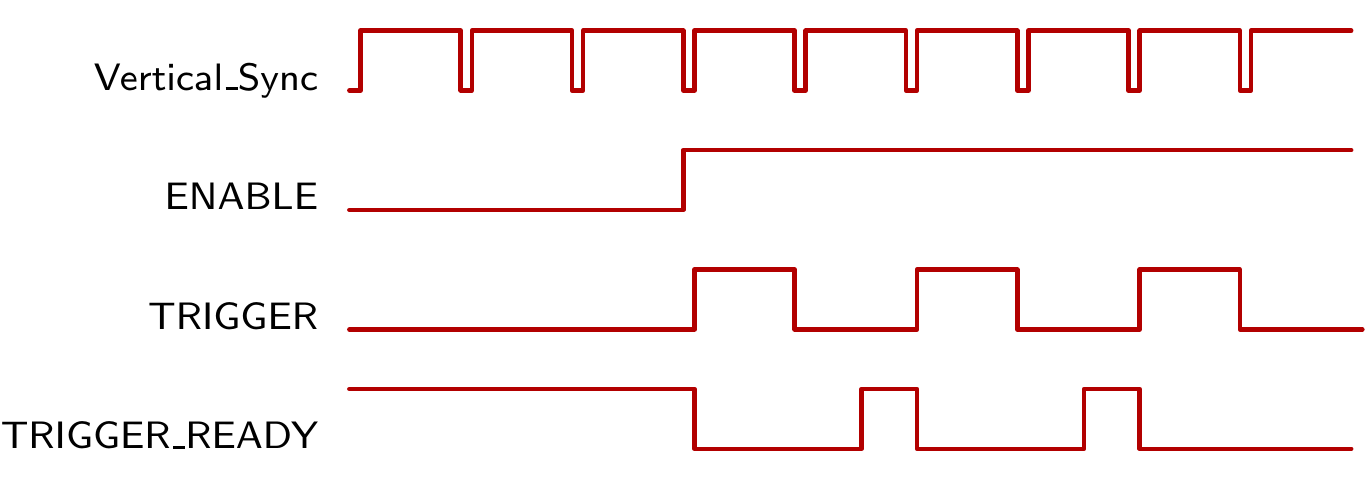
\includegraphics[width=\linewidth]{gpio.png}
  \caption{Timing diagram of the camera's IO signals}
  \label{Fig:5}
\end{figure}


%=======
%I_c[r,c,k] = [X_w[r,c,k], Y_w[r,c,k], Z_w[k], P[r,c,k]]
%\label{calEqn}
%\end{equation}
%where $r$ and $c$ are the pixel's row and column coordinate; $k$ is the step index for the current scan; $X_w[r,c,k]$ and $Y_w[r,c,k]$ are the CalTag grid coordinate at the intersection of the CalTag target's surface and the camera pixel's line-of-sight; $Z_w[k]$ is the Z-position of the rail; and $P[r,c,k]$ is the phase value of the projected PMP sequence in the line-of-sight of the camera pixel.  Once complete, we then have a 3D texture composed of a stack of 4-color digital images that are the height and width of our camera and $K$ layers deep with $P[r,c,k]$ ranging from $P_{min}[r,c]$ to $P_{max}[r,c]$ as $Z_w[k]$ ranges from $Z_{min}$ to $Z_{max}$.
%
%In order to parameterize the relationships between channels, let's define $\vec{x}_{r,c}$, $\vec{y}_{r,c}$, and $\vec{z}_{r,c}$ as the $K$-dimensional vector composed of $X_w[r,c,k]$, $Y_w[r,c,k]$, and $Z_w[k]$, and let's define $\vec{p}_{r,c}$ as the normalized phase coordinates derived from $P[r,c,k]$ according to:
%\begin{equation}
%\vec{p}_{r,c}[k] = \frac{P[r,c,k] - P_{min}[r,c]}{P_{max}[r,c] - P_{min}[r,c]}.
%\end{equation}
%From these vectors, we can derive a plot of any pixel channel versus any other channel.  For example, we can plot $\vec{x}_{r,c}$ versus $\vec{z}_{r,c}$ or, more importantly, $\vec{z}_{r,c}$ versus $\vec{p}_{r,c}$.  Assuming the pin-hole lens model for both the camera and the projector, we know from Liu~\textit{et al} that the relationship between $\vec{x}_{r,c}$ and $\vec{z}_{r,c}$ as well as $\vec{y}_{r,c}$ and $\vec{z}_{r,c}$ are given by the straight line relationships:
%\begin{eqnarray}
%\vec{x}_{r,c} & = & A_{r,c} \vec{z}_{r,c} + B_{r,c}, \mbox{ and} \\
%\vec{y}_{r,c} & = & C_{r,c} \vec{z}_{r,c} + D_{r,c},
%\label{pinHoleEqnXY}
%\end{eqnarray}
%where $A_{r,c}$, $B_{r,c}$, $C_{r,c}$, and $D_{r,c}$ are scalar constants representing the slope and intercepts found by best-fitting straight lines between recorded points; furthermore, the relationship between $\vec{z}_{r,c}$ versus $\vec{p}_{r,c}$ is given by the equation:
%\begin{equation}
%\tilde{z}[r,c] = \frac{E_{r,c} \vec{p}_{r,c} + F_{r,c}}{G_{r,c} \vec{p}_{r,c} + H_{r,c}},
%\label{pinHoleEqnPZ}
%\end{equation}
%where $E_{r,c}$, $F_{r,c}$, $G_{r,c}$, and $H_{r,c}$ are scalar constants found either through singular value decomposition~\cite{??} or the pseudo-inverse~\cite{??}. In situations where the lens of either the projector or the camera are not accurately modeled by the pin-hole lens model, we can replace eqn.~\eqref{pinHoleEqnPZ} with a more flexible fourth-order polynomial model defined as:
%\begin{equation}
%\tilde{z}[r,c] = E_{r,c} \vec{p}_{r,c}^{~4} + F_{r,c} \vec{p}_{r,c}^{~3} + G_{r,c} \vec{p}_{r,c}^{~2} + H_{r,c} \vec{p}_{r,c} + I_{r,c},
%\label{plyHoleEqn}
%\end{equation}
%where $E_{r,c}$, $F_{r,c}$, $G_{r,c}$, $H_{r,c}$, and $I_{r,c}$ are found using a least-squares polynomial fitting algorithm.  Equation~\eqref{pinHoleEqnXY} need not change since the line-of-sight of any camera pixel is a straight line regardless of any lens distortion.
%>>>>>>> 716b5f75bdda6aa6bf4630801fbe0c1071de81a3
%
%Now as an alternative to parameterizing our calibration data by eqns.~\eqref{pinHoleEqnXY}-\eqref{plyHoleEqn}, a wholly different approach is to build a 3D look-up-table indexed by the normalized phase values acquired during a scan. This is achieved by generating a set of plots between the world coordinates in $\vec{x}_{r,c}$, $\vec{y}_{r,c}$, and $\vec{z}_{r,c}$ versus $\vec{p}_{r,c}$ and then resampling them along equal increments of the $\vec{p}_{r,c}$ axis, keeping in mind that $\vec{x}_{r,c}$, $\vec{y}_{r,c}$, $\vec{z}_{r,c}$, and $\vec{p}_{r,c}$ are currently recorded along equal increments along $\vec{z}_{r,c}$.  Keeping in mind that this interpolation can be with greater or fewer samples, $L$, than the original collected data with $K$ layers.  Doing so, we define our look-up-table as a 3D texture according to:
%\begin{equation}
%LUT[r,c,l] = [X_w[r,c,l], Y_w[r,c,l], Z_w[r,c,l]]
%\end{equation}
%where $r$ and $c$ are the pixel's row and column coordinate and $l$ is the resampled step index replacing $k$. The benefits of using the look-up-table over the parameterized model is that it avoids the error associated with inappropriate parameterization of lens distortion as well as detrimental impact of phase distortions such as gamma~\cite{??} as well as dithering noise caused by using projector defocus to blur the pixels of a binary DMD pattern~\cite{??}. The only condition is that the phase image must be monotonic. With regards to real-time performance, the 3D look-up-table is easily implemented on an OpenGL shader using the {\em texture} function~\cite{??}.




%%%%%%%%%%%%%%%%%%%%%%%%%%%%%%%%%%%%%%%%%%%%%%%%%%%%%%%%%%%%%
%%%%% References %%%%%
\acknowledgments
This work has been supported by Intel Corporation and the National Science Foundation under contract No. 1539157 and the Visual and Experiential Computing initiative. Dr.~Daniel~L.~Lau is a Professor at the University of Kentucky and a Founder of Seikowave Inc., a private company that designs and sells structured light scanners.

\bibliography{report}   %>>>> bibliography data in report.bib
\bibliographystyle{spiebib}   %>>>> makes bibtex use spiebib.bst

\end{document} 
